\subsection{Criteria for the orbital height of the satellites}
\paragraph{Satellites currently in Orbit\\}
If only geometric considerations were to be applied in the design of a satellite constellation, it is clear that the higher the orbit the broader is the footprint in the surface leading to a smaller number of satellites. However, if the service of communications is to be offered, the satellites currently in orbit or in design phases need to be at higher orbit than the one of the constellation. The purpose of that requirement is to intersect the field of view of the satellites that nowadays point to Earth.

From source [?] we can study how the currently on orbit satellites are launched and specially, in which orbits. The results of the study of this source is presented below. All of them are in Low Earth Orbits, and half of them above 550km. In total, there are 203 operational satellites.

\begin{figure}[H]
	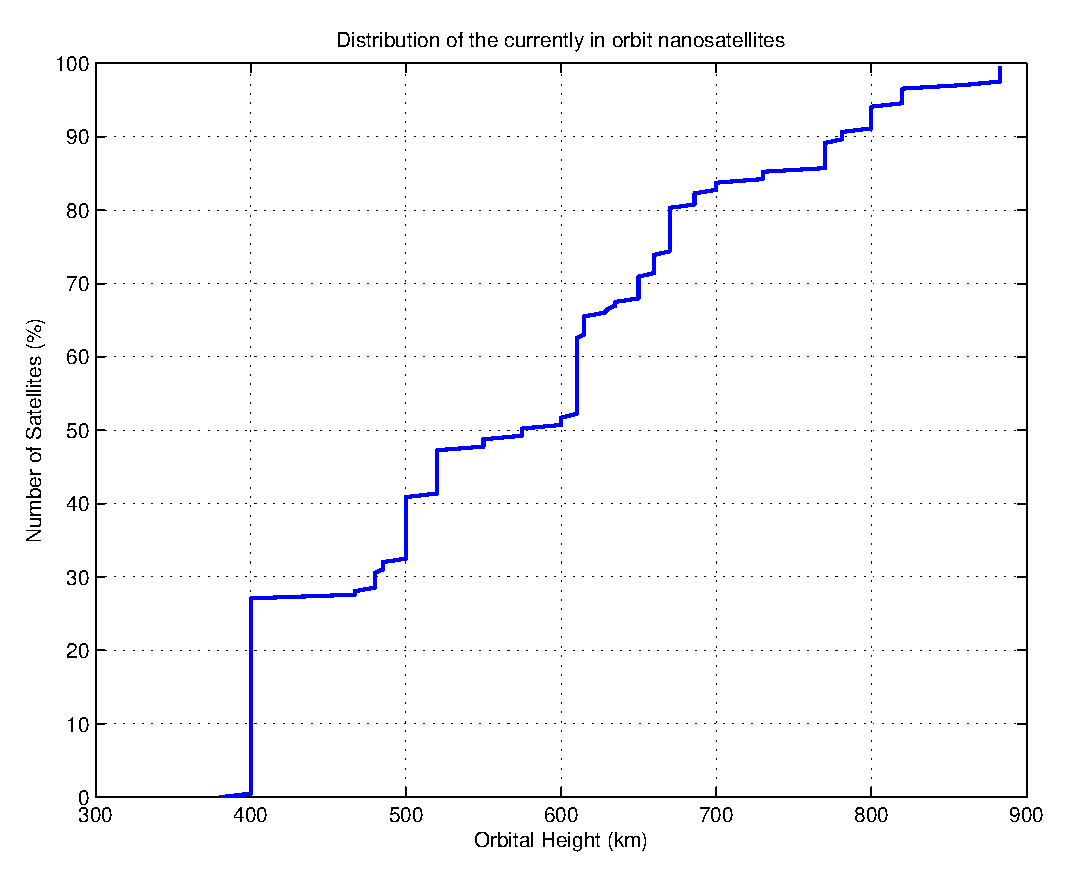
\includegraphics[scale=0.8]{CurrentOrbitDistribution}
	\caption{Distribution of the currently in orbit nanosatellites.}	
\end{figure}

\newpage

\paragraph{The most interesting potential clients\\}
Lots of satellites are orbiting at heights lower than 500km, mainly because one of the most feasible way of launching a small satellite is from the International Space Station. However, this very low LEOs are related to very high speeds and specially to low lifetimes, since drag affects them in a more significant way. To the interest of the constellation, the satellites at higher altitudes are a better commercial target, since they are going to be in orbit for longer missions. In addition, the same orbit decay problems are avoided for the constellation satellites.

\subsection{New Space: Adapting to new society needs}
Nowadays new satellites willing to provide services to Earth are being positioned closer than ever. Where closer can be applied in many points of view. Physically, the satellites are placed every time at lower orbits, since the energetic requirement is lower. Technically, the space certified materials and hardware are becoming more feasible, and new launchers are smaller. In the end, everything comes down to an economic approach, launching satellites is becoming cheaper every time and this means closer to the private pocket.\\
\newline
In the future, the possibility of using the Astrea constellation to contact Earth can reduce the requirements for the antennas and AOCSs to communicate with ground, leading to a whole new level of resources for the satellite payload. For instance, by communicating to the constellation pointing to outter space instead of pointing down to Earth. That is just a way in which Astrea is in the New Space Generation.\\
\newline
\textbf{In conclusion,} In the decision process one of the statistics considered with certain weight will be the following: the ratio of satellites at which the constellation will be able to provide service considering that nowadays all of them point down to Earth. 